\documentclass{beamer}
\usepackage{listings}
\lstset
{
language=C,
frame=single, 
breaklines=true,
columns=fullflexible
}
\usepackage{subcaption}
\usepackage{url}
\usepackage{tikz}
\usepackage{graphicx}
\usepackage{multicol}
\usepackage{tkz-euclide} % loads  TikZ and tkz-base
%\usetkzobj{all}
\usetikzlibrary{calc,math}
\usepackage{float}
\usepackage{amsthm}
\newcommand\norm[1]{\left\lVert#1\right\rVert}
\renewcommand{\vec}[1]{\mathbf{#1}}
\newcommand{\R}{\mathbb{R}}
\newcommand{\C}{\mathbb{C}}
\newcommand{\comb}[2]{{}^{#1}\mathrm{C}_{#2}}
\providecommand{\brak}[1]{\ensuremath{\left(#1\right)}}
\providecommand{\abs}[1]{\vert#1\vert}
\providecommand{\fourier}{\overset{\mathcal{F}}{ \rightleftharpoons}}
\providecommand{\sbrak}[1]{\ensuremath{{}\left[#1\right]}}
\usepackage[export]{adjustbox}
\usepackage[utf8]{inputenc}
\usepackage{amsmath}
\usepackage[version=4]{mhchem}
\usetheme{Boadilla}
\title{GATE 2021 (ST), Q.15}
\author{V Rahul}
\institute{IITH}
\date{\today}
\begin{document}
\begin{frame}
    \titlepage
\end{frame}
\begin{frame}{Question}
    \begin{block}{GATE 2021 (ST), Q.15}
        A fair die is rolled twice independently. Let X and Y denote the outcomes of the first and second roll, respectively. Then $E(X+Y\:|\:(X-Y)^2=1)$ equals
    \end{block}
\end{frame}
\begin{frame}{PDF of X+Y}
    \begin{block}{}
        PDF of sum of random variables X and Y given their individual PDFs can be calculated using
        \begin{enumerate}
            \item Convolution
            \item Characteristic Function
        \end{enumerate}
    \end{block}
\end{frame}
\begin{frame}{PDF of X and Y}
    \begin{block}{}
        X and Y are two independent random variables that can take the values 1, 2, 3, 4, 5, 6.
        \begin{align}
            \Pr\brak{X=k}=\frac{1}{6}, 1\leq k \leq 6\\
            \Pr\brak{Y=k}=\frac{1}{6}, 1\leq k \leq 6
        \end{align}
    \end{block}
\end{frame}
\begin{frame}{Convolution}
    \begin{block}{}
        The general formula for the distribution of the sum Z=X+Y of two discrete random variables is
        \begin{align}
            \Pr\brak{Z=z} = \sum_{k=-\infty}^{\infty} \Pr\brak{X=k,Y=z-k}
        \end{align}
        If X and Y are independent,
        \begin{align}
            \Pr\brak{Z=z} = \sum_{k=-\infty}^{\infty} \Pr\brak{X=k}\times\Pr\brak{Y=z-k}
        \end{align}
        The counterpart for independent continuous random variables X and Y with probability density functions f(x), g(x) is
        \begin{align}
            \Pr\brak{Z=z}=\int_{-\infty}^{+\infty} x\times f(t)\times g(z-t)dt
        \end{align}
    \end{block}
\end{frame}
\begin{frame}{PDF of X+Y using convolution}
    \begin{block}{}
        $\Pr\brak{X+Y=n}$
        \begin{align}
            =&\sum_{k=n-6}^{n-1} \Pr\brak{X=k}\times\Pr\brak{Y=n-k}, 1\leq k \leq 6\\
            =&\sum_{k=n-6}^{n-1} \frac{1}{6}\times\frac{1}{6}, 1\leq k \leq 6\\
            =&\sum_{k=n-6}^{n-1} \frac{1}{36}, 1\leq k \leq 6\\
            =&
            \left\{
	        \begin{array}{ll}
		        \frac{n-1}{36}  & ,\: 2 \leq n \leq 7 \smallskip\\
		        \frac{13-n}{36} & ,\: 8 \leq n \leq 12
	        \end{array}
            \right.\label{0.0.8}
        \end{align}
    \end{block}
\end{frame}
\begin{frame}{PDF of X+Y using convolution}
    \begin{figure}[htb]
        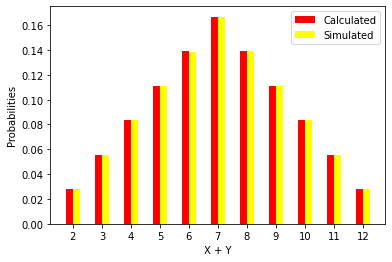
\includegraphics[width=0.8\columnwidth]{Assignment-4(1).png}
        \caption{Plot of PMF for X+Y}
    \end{figure}
\end{frame}
\begin{frame}{PDF of X-Y using convolution}
    \begin{block}{}
        $\Pr\brak{X-Y=n}$
        \begin{align}
            =&\sum_{k=n+1}^{n+6} \Pr\brak{X=k}\times\Pr\brak{Y=k-n}, 1\leq k \leq 6\\
            =&\sum_{k=n+1}^{n+6} \frac{1}{6}\times\frac{1}{6}, 1\leq k \leq 6\\
            =&\sum_{k=n+1}^{n+6} \frac{1}{36}, 1\leq k \leq 6\\
            =&
            \left\{
	        \begin{array}{ll}
		        \frac{n+6}{36} & ,\: -5 \leq n \leq 0 \smallskip\\
		        \frac{6-n}{36} & ,\: 1  \leq n \leq 5
	        \end{array}
            \right.\label{0.0.12}
        \end{align}
    \end{block}
\end{frame}
\begin{frame}{PDF of X-Y using convolution}
    \begin{figure}[htb]
        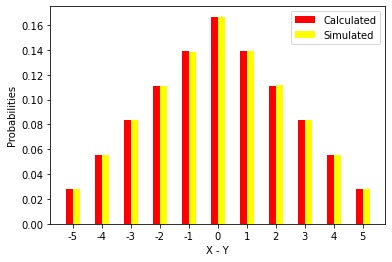
\includegraphics[width=0.8\columnwidth]{Assignment-4(2).png}
        \caption{Plot of PMF for X-Y}
    \end{figure}
\end{frame}
\begin{frame}{Expectation value}
    \begin{block}{Definition}
        \begin{enumerate}
            \item The expectation value of X is often called as mean of X and is denoted by $\mu_x$.
            \item It is often considered as measure of central tendency.
        \end{enumerate}
    \end{block}
    \begin{block}{Formulas}
        For discrete random variable X,
        \begin{align}
            E\brak{X}=\sum x_{i}\times\Pr\brak{X=x_{i}}
        \end{align}
        For continuous random variable X having probability density function $f(x)$,
        \begin{align}
            E\brak{X}=\int_{-\infty}^{+\infty} x\times f(x)dx
        \end{align}
    \end{block}
\end{frame}
\begin{frame}{Expectation value}
    \begin{block}{Formulas}
        If X and Y are two discrete random variables,
        \begin{align}
            E\brak{g(x,y)}=\sum^{\infty}_{i=-\infty}\sum^{\infty}_{j=-\infty}\,g(x_i,y_i)\times \Pr\brak{X=x_i,Y=y_i}
        \end{align}
        If X and Y are two continuous random variables having joint density function $f(x,y)$,
        \begin{align}
            E\brak{g(x,y)}=\int_{-\infty}^{\infty}\int_{-\infty}^{\infty} g(x,y) \times f(x,y)dxdy
        \end{align}
    \end{block}
\end{frame}
\begin{frame}{Expectation value}
    \begin{block}{Properties}
        If c is any constant, then
        \begin{align}
            E\brak{cX}=c\timesE\brak{X}
        \end{align}
        If X and Y are any random variables, then
        \begin{align}
            E\brak{X + Y} = E\brak{X} + E\brak{Y}
        \end{align}
        If X and Y are independent random variables, then
        \begin{align}
            E\brak{XY} = E\brak{X} \times E\brak{Y}
        \end{align}
    \end{block}
\end{frame}
\begin{frame}{Solution contd.}
    \begin{block}{Conditional Probability}
        \Pr\brak{X|Y}=\frac{\Pr\brak{X,Y}}{\Pr\brak{Y}}
        \end{block}
    \begin{block}{}
        $E\brak{X+Y\:|\:(X-Y)^2=1}$
        \begin{align}
            =&\sum\:n\times\Pr\brak{X+Y=n\:|\:(X-Y)^2=1}\\
            =&\sum\:n\times\frac{\Pr\brak{X+Y=n,(X-Y)^2=1}}{\Pr\brak{(X-Y)^2=1}}
        \end{align}
    \end{block}
\end{frame}
\begin{frame}{Solution contd.}
    \begin{block}{}
        $E\brak{X+Y\:|\:(X-Y)^2=1}$
        \begin{align}
            \begin{split}
                =\sum\:n\times\frac{\Pr\brak{X+Y=n,(X-Y)=1}}{\Pr\brak{(X-Y)=1}}
                \bigskip\\
                \times\Pr\brak{(X-Y)=1|(X-Y)^2=1}
                \bigskip\\
                +\sum\:n\times\frac{\Pr\brak{X+Y=n,(X-Y)=-1}}{\Pr\brak{(X-Y)=-1}}
                \bigskip\\
                \times\Pr\brak{(X-Y)=1\:|\:(X-Y)^2=1}
                \end{split}
                \\
                \begin{split}
                =\:\frac{\Pr\brak{(X-Y)=1\:|\:(X-Y)^2=1}}{\Pr\brak{(X-Y)=1}}
                \bigskip\\
                \times\sum\:n\times\Pr\brak{X+Y=n,(X-Y)=1}
                \bigskip\\
                +\frac{\Pr\brak{(X-Y)=-1\:|\:(X-Y)^2=1}}{\Pr\brak{(X-Y)=-1}}
                \bigskip\\
                \times\sum\:n\times\Pr\brak{X+Y=n,(X-Y)=-1}\label{0.0.18}
            \end{split}
        \end{align}
    \end{block}
\end{frame}
\begin{frame}{Solution contd.}
    \begin{block}{}
        Using equations \eqref{0.0.8} and \eqref{0.0.12} in \eqref{0.0.18}\\
        We get,\\
        \newline
        $E\brak{X+Y\:|\:(X-Y)^2=1}$
        \begin{align}
            =&\:\brak{\frac{\frac{1}{2}}{\frac{5}{36}}}\times\brak{\frac{35}{36}}+\brak{\frac{\frac{1}{2}}{\frac{5}{36}}}\times\brak{\frac{35}{36}}\\
            =&\:7
        \end{align}
    \end{block}
\end{frame}
\end{document}